\section{Pokemon mechanics}
\label{sec:pokemon-mechanics}

The Pokemon games are home to a vast amount of mechanics. In order to fully understand
this project, it is important to have a basic understanding of the mechanics present in a Pokemon battle.

The following section aims to briefly explain these mechanics.

\subsection{Type chart}
A Pokemon will under normal circumstances have 1 or 2 types that represents its elemental alignment and similarly a Pokemon move will have 1 type.
Each type determines its effectiveness against other types. The effectivenesses are categorized as follows:
\begin{itemize}
  \item No effect (0x multiplier)
  \item Not very effective (0.5x multiplier)
  \item Effective (1x multiplier)
  \item Super effective (2x multiplier)
\end{itemize}
These multipliers are stacking, so if a Pokemon has 2 types that resists an incoming attack, the multiplier becomes $ 0.5*0.5=0.25 $.
\notebox{Example: A fire type Pokemon, Charmander, is in a battle with the water type Pokemon, Squirtle.
  The Squirtle uses the water type move Water Gun against the Charmander. As water is super effective against fire, the move
  Water Gun receives a 2x multiplier to its damage.}

For the full list of type advantages and disadvantages, see appendix \ref{appendix:type-chart}.

\subsection{Stats}
A Pokemons power is determined by its stats. Since generation 2 a Pokemon has been described by the following stats:
\begin{itemize}
  \item HP: Determines the amount of hit points a Pokemon has. The more hit points a Pokemon has, the more durable it is.
  \item Attack: Determines the power of physical attacking moves.
  \item Defense: Determines a Pokemons resistance to physical attacking moves.
  \item Special Attack: Determines the power of special attacking moves.
  \item Special Defense: Determines a Pokemons resistance to special attacking moves.
  \item Speed: Determines a Pokemons speed, which is used to determine who goes first in a round of battle.
\end{itemize}
A Pokemons stats are influenced by a few factors: its base stats, level, nature, individual values and effort values.
Together they compose the Pokemons actual stats.

\subsubsection{IVs and EVs}
Individual values \cite{IndividualValues} and effort values \cite{EffortValues} (referred to as IVs and EVs) are hidden values attributed to a Pokemon to create variety in each Pokemons power levels within its species.
When a Pokemon is encountered it will be generated with IVs ranging from 0-31 for each of its stats. A higher IV will result in a higher total stat.

EVs are values gained through battles. A Pokemon can have a total number of 510 EVs with a limit of 255 points per stat.

\subsubsection{Natures}
A Pokemons nature \cite{Natures} is determined when it is generated. A nature gives a Pokemon a ±10\% modifier to select stats.
If a nature both raises and lowers a stat it is called a "Neutral nature" and no changes will occur to the final stat.
Please refer to table \ref{tab:nature-table} for the full list of natures and their effects.
\begin{figure}[h]
  \centering
  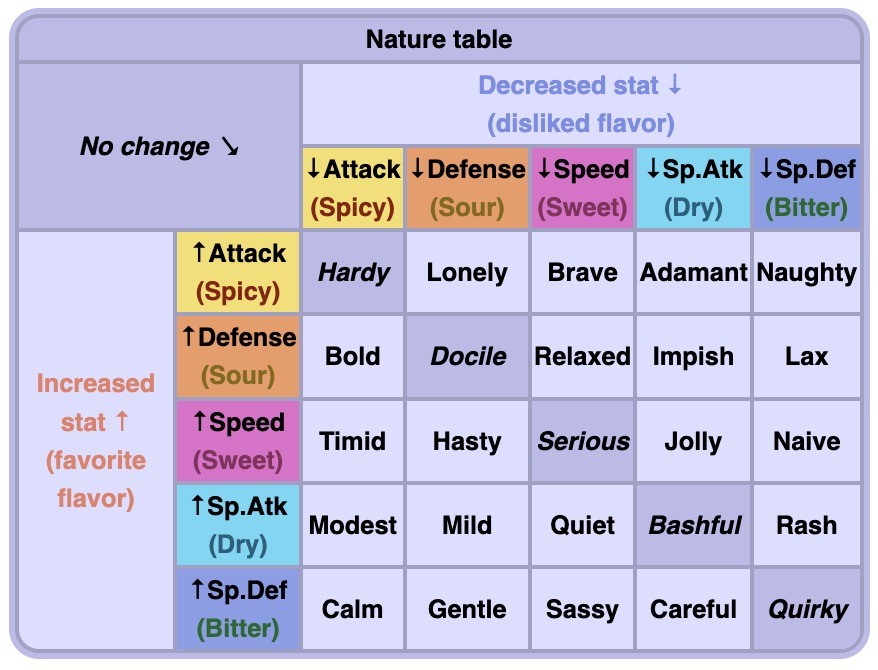
\includegraphics[width=.8\textwidth]{assets/nature-stat-table.jpg}
  \label{tab:nature-table}
  \caption{Table of Natures and how they affect stats from Bulbapedia \cite{Natures}}
\end{figure}

\subsubsection{Stat boosts}
Stat boosts are temporary modifiers applied to a Pokemons stat in combat. A stat is raised and lowered in stages ranging from -6 to +6 \cite{StatBoosts}.
Certain moves or abilites can raise or lower a Pokemons stat in stages. By default all stats begin at stage 0, meaning no change.

\begin{figure}[h]
  \centering
  \scalebox{.8}{
    \begin{tabular}{|c|c|c|c|c|c|c|c|c|c|c|c|c|c|}
      \hline
      \textbf{Stage}    & -6    & -5    & -4    & -3    & -2    & -1    & 0     & +1    & +2    & +3    & +4    & +5    & +6    \\
      \hline
      \textbf{Modifier} & $2/8$ & $2/7$ & $2/6$ & $2/5$ & $2/4$ & $2/3$ & $2/2$ & $3/2$ & $4/2$ & $5/2$ & $6/2$ & $7/2$ & $8/2$ \\
      \hline
    \end{tabular}
  }
  \label{tab:stat-stage-modifiers}
  \caption{Table of stat stages and their modifier from Bulbapedia \cite{StatBoosts}}

\end{figure}

\subsubsection{Formula}
With the above sections in mind, the final stat value of a Pokemon can be calculated using the following formulas \cite{PokemonStats}.
Please note that the HP stat has a different formula compared to the other stats.

\begin{figure}
  $$
    HP = \left\lfloor \frac{(2 * Base + IV + \left\lfloor \frac{EV}{4} \right\rfloor) * Level}{100} \right\rfloor + Level + 10
  $$
  
  $$
    OtherStat = \left\lfloor \left( \left\lfloor \frac{(2 * Base + IV + \left\lfloor \frac{EV}{4} \right\rfloor) * Level}{100} \right\rfloor + 5 \right) * NatureMod \right\rfloor
  $$
  \label{formula:stat-formula}
  \caption{Formulas for calculating a Pokemons stats \cite{PokemonStats}}
\end{figure}

\subsection{Abilites}
\subsection{Held items}
\subsection{Status conditions}
\subsubsection{Poison}
\subsubsection{Burn}
\subsubsection{Sleep}
\subsubsection{Paralysis}
\subsubsection{Freeze}
\subsubsection{Confusion}
\subsubsection{Flinch}
\subsubsection{Seed}
\subsubsection{Infatuation}
\subsubsection{Curse}
\subsubsection{Nightmare}
\subsection{Moves}
% Power
% Damage range
% OHKO
% Critical hits
% Physical/Special
% Accuracy
% Priority
% Targeting
\subsection{Weather}
\subsection{Field effects}
\subsection{Battles}
% Turn order
\subsubsection{Double battles}
\subsubsection{Special battles}
\subsection{Special mechanics}
\subsubsection{Mega Evolution}
\subsubsection{Z-moves}
\subsubsection{Dynamax and Gigantomax}
\subsubsection{Terastalization}
